% Inspiré de http://en.wikibooks.org/wiki/LaTeX/Title_Creation
\begin{center}
	\begin{minipage}[t]{0.48\textwidth}
	  \begin{flushleft}
	    
\includegraphics [width=30mm]{img/logo_kth.jpg} \\[0.1cm]
		Kungliga Tekniska Högskolan\\
		Valhallavägen 79\\
		100 44 Stockholm
	  \end{flushleft}
	\end{minipage}
	\begin{minipage}[t]{0.48\textwidth}
	  \begin{flushright}
	  \end{flushright}
	\end{minipage} \\[1cm]

	\textsc{\Large \reportsubject}\\[0.3cm]
	\HRule \\[0.4cm]
	{\Huge \bfseries \reporttitle}\\[0.3cm]
	{\LARGE \bfseries «~\stagetopic~»}\\[0.3cm]
	{\Large \dateperiod}\\[0.4cm]
	\HRule \\[1.5cm]

	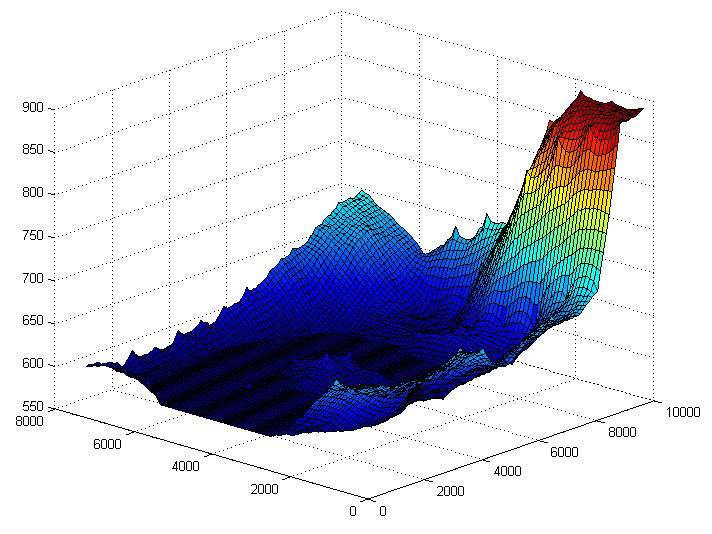
\includegraphics [width=0.55\linewidth]{img/icon.jpg} \\[1.5cm]
	\begin{minipage}[t]{0.5\textwidth}
	  \begin{flushleft} \large
	    \emph{Authors}\\
	    \reportauthor
	  \end{flushleft}
	\end{minipage}
	\begin{minipage}[t]{0.4\textwidth}
	  \begin{flushright} \large
	    \emph{Teacher} \\
	    \enseignants
	  \end{flushright}
	\end{minipage}

	\vfill
	\footnotesize{Scholar year 2014-2015}
\end{center}
